\textnormal{
We have implemented this approach using Python 3 and Jupyter Notebook. The file `Huffman\_User\_Command.ipynb' is used to compress the files based on the user commands. On running this file we have to input the master file which is used to generate the encoding table. This table is generated by calculating the frequency of each character in the master data file (`data.txt'). Then the user will have to choose the option of either compress/decompress/exit. On choosing compress/decompress the user will have to enter the file name to be compressed or decompressed. The input for the compression will have to be a text file and the file for decompression is an already compressed binary file. The code file continues to prompt the user to enter the subsequent actions to be taken. The user can exit from this application by entering exit in the console for action to be taken. After each compression or decompression we will get a status message(success/fail). If the action is successful then the code will aslo display the name of the compressed/decompressed file.
\\
The file `Huffman\_Encoding\_Demo.ipynb' file is used to show a demo and it does not take user inputs. The code is written to take the `data.txt' file and generate the encoding table. The encoding table generated is saved as a pickle object in the local folder. The encoding table contains the Huffman codes for each character in the master data file. This table is used to compress the subsequent data files for similar types. The code takes the `sample.txt' file and compresses it using the encoding table generated from `data.txt'. The encoded file is saved as `sample1\_compressed.bin', a binary file. The size of the compressed file is also displayed.The next step is to compare the compression ratio achieved using the original approach and the new approach. So now for the original method the encoding table is changed and the compression is performed again. Finally the 2 compression ratios are displayed. In this step we find that the compression ratio using the new approach is not optimal which was expected and the 2 compression ratios are not that different. Moreover the header for the file using our approach is larger than the original method.Now when we try to compress the next file `sample2.txt', the compression using our method is faster and this time we dont have to send the header. On combining the compresed file and the headers, we find that the compression using our new approach works better than the original method.
\\
One of the errors that we may encouter in our file is that if the sample file to be compressed contains a new character that was not present in the original master data file. The screenshot for which is given below:
\\*
\begin{figure}[!h]
    \centering
    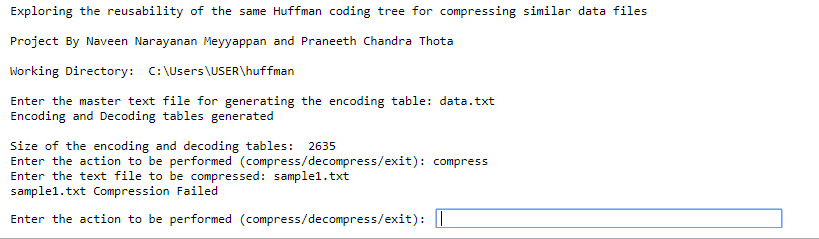
\includegraphics[width=90mm,scale=0.5]{Capture3.png}
    \caption{Error Message}
\end{figure}
\\*
\\On compressing the 10 sample files using the 2 methods we found that the total size of the compressed files including the headers using the original approach is 38627 bytes and 34012 bytes using the new approach. On the whole we have achieved higher compression and also the compression using our method is faster. Thereby we conclude that this method serves as a faster alternative for the original huffman compression. Moreover this method reduces the time and complexity of the algorithm.
}
